\chapter{Proposed method}
% Talk about the goal (compare methods for timeseries classification)
The goal of this thesis is to compare different methods for time series classification with missing data.
To conduct this comparison, we implemented several machine learning models and compared their performance on a dataset of Satellite Image Time Series.

\section{Fair comparison}
% How to make fair experiments:\\
%   - k-folds different seeds\\
%   - same metrics (accuracy)\\
%   - organize results (wandb)
To ensure a fair comparison, we used the same dataset and the same metrics for all the models.
The dataset we used is the Satellite Image Time Series (SITS) dataset, which contains 137,606 time series of satellite images of natural and semi-natural areas. 
The data available for this task is not so abundant, so we used k-fold cross validation with $k=5$ and different seeds to ensure that the results were not biased by the partitioning of the dataset.
When splitting the dataset into training/validation/test, we ensured that the classes were balanced in each fold and that there was no spatial correlation, avoiding placing the same polygon pixels in the same sets.

\begin{table}[H]
  \centering
  \begin{tabular}{lllllll}
  \hline
  Class   & \multicolumn{2}{l}{Train} & \multicolumn{2}{l}{Validation} & \multicolumn{2}{l}{Test} \\ \cline{2-7} 
          & Pixels  & (\%) & Pixels    & (\%)    & Pixels & (\%) \\ \hline
  Built   & 6,381   & 8.1             & 1,775     & 6.1                & 2,256  & 7.7             \\
  Road    & 3,014   & 3.8             & 1,323     & 4.5                & 828    & 2.8             \\
  Water   & 16,534  & 20.9            & 6,856     & 23.4               & 8,705  & 29.8            \\
  Forest  & 29,654  & 37.4            & 10,739    & 36.7               & 8,782  & 30.1            \\
  Vine    & 16,399  & 20.7            & 6,002     & 20.5               & 6,266  & 21.5            \\
  Orchard & 1,464   & 1.8             & 218       & 0.7                & 393    & 1.3             \\
  Crop    & 2,598   & 3.3             & 1,370     & 4.7                & 1,237  & 4.2             \\
  Other   & 3,147   & 4.0             & 966       & 3.3                & 699    & 2.4             \\ \hline
  Total   & 79,191  & 100             & 29,249    & 100                & 29,166 & 100            
  \end{tabular}
  \caption{Distribution of classes, polygons and pixels for each dataset.}
\end{table}

The metrics that we used to evaluate the models were the classification accuracy of the models.

In order to keep track of the experiments, we used Weights and Biases (wandb) to log the configuration and the results of the experiments.
This was very useful to compare the results of the different models. It also helped to keep the models reproducible and to fine-tune the hyperparameters of the models.

\section{Models}
% Pick models\\
% - read paper\\
%  - check for source code\\
%  - adapt/update code\\
First, we looked at the state of the art in time series classification in order to select the most promising models.
Then I studied the papers, checked if any source code was available and then implemented or adapted the code to our needs.

% -- tensorflow vs pytorch\\
With the exception of the transformers, all the models have been implemented using TensorFlow, while the transformers have been implemented using PyTorch.
% short tensorflow vs pytorch?

For almost every model we implemented, we also developed a baseline model that did not handle missing data.
This baseline model was used to compare the performance of the models that handled missing data.
For each model we tried different things to improve the performance, such as changing the hyperparameters or changing the architecture of the network.
 
% - experiments\\
% -- hyperparameters\\
% -- architecture\\

% TODO
- early stopping\\

\section{Weights and Biases}
% TODO: talk about wandb

\begin{figure}[H]
  \centering
  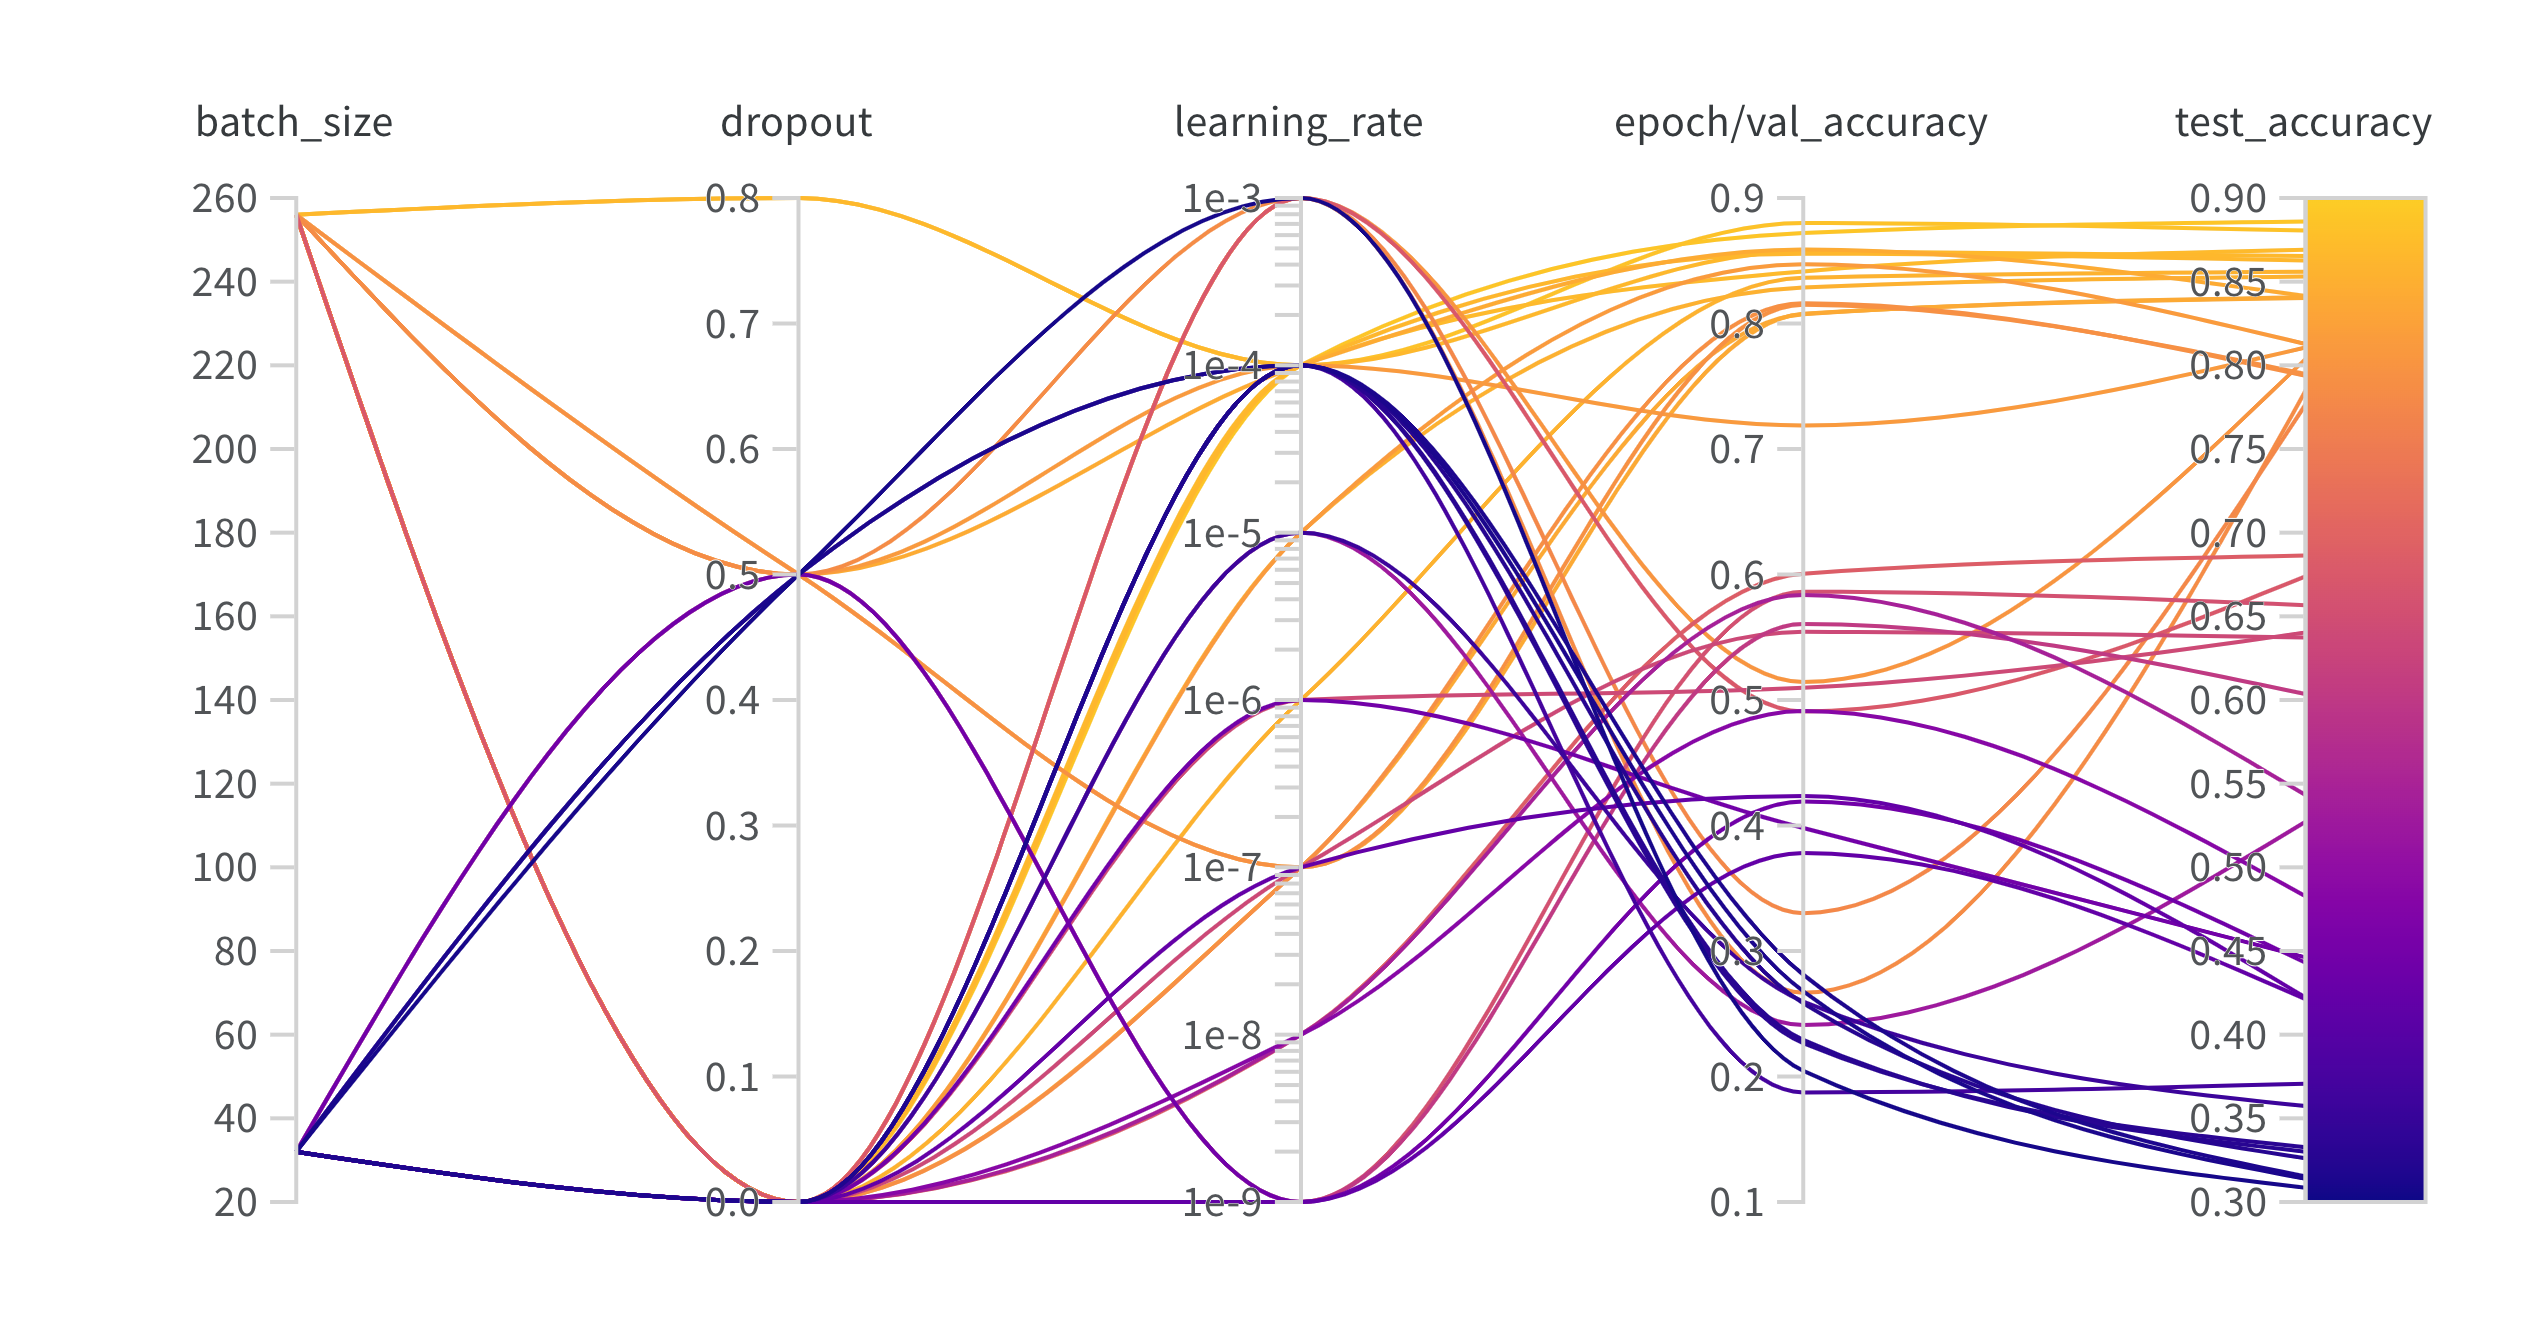
\includegraphics[width=0.9\textwidth]{wandb1}
  \caption{Example of parallel cordinates plot in wandb}
\end{figure}

\begin{figure}[H]
  \centering
  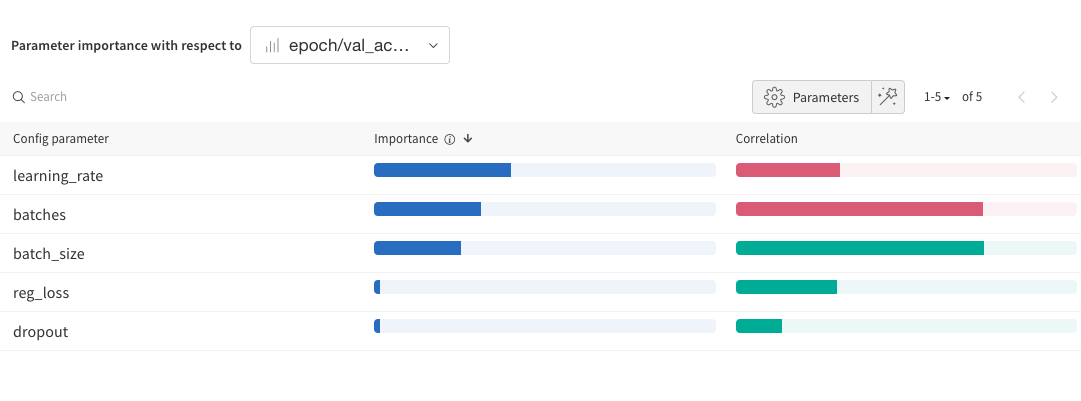
\includegraphics[width=0.9\textwidth]{wandb2}
  \caption{Example of Parameter importance panel in wandb}
\end{figure}




